%SETUP%
\documentclass{scrreprt}
\usepackage [T1] {fontenc}
\usepackage [utf8] {inputenc}
\usepackage{fancyhdr} % for headers + footers control
\usepackage[ngerman]{babel} % set german language
\usepackage{graphicx} % for images
% \usepackage{svg} % for vector graphics
\usepackage{wrapfig} % for float images
\usepackage[a4paper]{anysize}
\usepackage{lmodern} % Latin modern font
\usepackage{float} % for better floating of objects
\usepackage{units}
\usepackage[font=small,labelfont=bf,hang]{caption}
\usepackage{subcaption} 

\usepackage[table,xcdraw]{xcolor} % for colorful tables
% ams 
\usepackage{amsmath}
\usepackage{amssymb}
\usepackage{amsfonts}
% turn on or off:
\usepackage [colorlinks=true] {hyperref} % colorful internal links

\usepackage[square,sort,comma,numbers]{natbib} % for cites

\marginsize{2cm}{2cm}{1cm}{1cm}



\begin{document}
\author{Jannes Brunner}
\title{AWE Belegarbeit SS 2017}

	\begin{titlepage}
		\begin{center}
			{\large Belegarbeit}\\
			{\large Berlin, XX.XX.201X}
			\vspace{0.5cm} \hrule \vspace{0.6cm}
			{\huge AWE: \\ Wissenschaftliches Arbeiten mit LaTeX \\}
			\vspace{0.8cm}
			\begin{figure}[h!]
				\centering
				
\includegraphics[width=0.5\textwidth]{images/HTW_Logo_rgb.png}
			\end{figure}
		
			\vspace{0.8cm}
			\large {Jannes Brunner}
		\end{center}
		\vspace{0.6cm}
		{\textbf Abstract}: Computer Science
	
		
	\end{titlepage}
	
	\tableofcontents
	
	\chapter{Texte}
	\section{Text mit 1000 Wörtern \cite{ref1}} 
	Eine wunderbare Heiterkeit hat meine ganze Seele eingenommen, gleich den süßen Frühlingsmorgen, die ich mit ganzem Herzen genieße. Ich bin allein und freue mich meines Lebens in dieser Gegend, die für solche Seelen geschaffen ist wie die meine. Ich bin so glücklich, mein Bester, so ganz in dem Gefühle von ruhigem Dasein versunken, daß meine Kunst darunter leidet. Ich könnte jetzt nicht zeichnen, nicht einen Strich, und bin nie ein größerer Maler gewesen als in diesen Augenblicken. Wenn das liebe Tal um mich dampft, und die hohe Sonne an der Oberfläche der undurchdringlichen Finsternis meines Waldes ruht, und nur einzelne Strahlen sich in das innere Heiligtum stehlen, ich dann im hohen Grase am fallenden Bache liege, und näher an der Erde tausend mannigfaltige Gräschen mir merkwürdig werden; wenn ich das Wimmeln der kleinen Welt zwischen Halmen, die unzähligen, unergründlichen Gestalten der Würmchen, der Mückchen näher an meinem Herzen fühle, und fühle die Gegenwart des Allmächtigen, der uns nach seinem Bilde schuf, das Wehen des Alliebenden, der uns in ewiger Wonne schwebend trägt und erhält; mein Freund! Wenn’s dann um meine Augen dämmert, und die Welt um mich her und der Himmel ganz in meiner Seele ruhn wie die Gestalt einer Geliebten – dann sehne ich mich oft und denke : ach könntest du das wieder ausdrücken, könntest du dem Papiere das einhauchen, was so voll, so warm in dir lebt, daß es würde der Spiegel deiner Seele, wie deine Seele ist der Spiegel des unendlichen Gottes! – mein Freund – aber ich gehe darüber zugrunde, ich erliege unter der Gewalt der Herrlichkeit dieser Erscheinungen. Eine wunderbare Heiterkeit hat meine ganze Seele eingenommen, gleich den süßen Frühlingsmorgen, die ich mit ganzem Herzen genieße. Ich bin allein und freue mich meines Lebens in dieser Gegend, die für solche Seelen geschaffen ist wie die meine. Ich bin so glücklich, mein Bester, so ganz in dem Gefühle von ruhigem Dasein versunken, daß meine Kunst darunter leidet. Ich könnte jetzt nicht zeichnen, nicht einen Strich, und bin nie ein größerer Maler gewesen als in diesen Augenblicken. Wenn das liebe Tal um mich dampft, und die hohe Sonne an der Oberfläche der undurchdringlichen Finsternis meines Waldes ruht, und nur einzelne Strahlen sich in das innere Heiligtum stehlen, ich dann im hohen Grase am fallenden Bache liege, und näher an der Erde tausend mannigfaltige Gräschen mir merkwürdig werden; wenn ich das Wimmeln der kleinen Welt zwischen Halmen, die unzähligen, unergründlichen Gestalten der Würmchen, der Mückchen näher an meinem Herzen fühle, und fühle die Gegenwart des Allmächtigen, der uns nach seinem Bilde schuf, das Wehen des Alliebenden, der uns in ewiger Wonne schwebend trägt und erhält; mein Freund! Wenn’s dann um meine Augen dämmert, und die Welt um mich her und der Himmel ganz in meiner Seele ruhn wie die Gestalt einer Geliebten – dann sehne ich mich oft und denke : ach könntest du das wieder ausdrücken, könntest du dem Papiere das einhauchen, was so voll, so warm in dir lebt, daß es würde der Spiegel deiner Seele, wie deine Seele ist der Spiegel des unendlichen Gottes! – mein Freund – aber ich gehe darüber zugrunde, ich erliege unter der Gewalt der Herrlichkeit dieser Erscheinungen. Eine wunderbare Heiterkeit hat meine ganze Seele eingenommen, gleich den süßen Frühlingsmorgen, die ich mit ganzem Herzen genieße. Ich bin allein und freue mich meines Lebens in dieser Gegend, die für solche Seelen geschaffen ist wie die meine. Ich bin so glücklich, mein Bester, so ganz in dem Gefühle von ruhigem Dasein versunken, daß meine Kunst darunter leidet. Ich könnte jetzt nicht zeichnen, nicht einen Strich, und bin nie ein größerer Maler gewesen als in diesen Augenblicken.
	
	 Wenn das liebe Tal\footnote{Ein Tal ist eine durch das Wechselspiel von Erosion und Denudation entstandene, für gewöhnlich langgestreckte, nach mindestens einer Seite offene Hohlform in der Landschaft.} um mich dampft, und die hohe Sonne an der Oberfläche der undurchdringlichen Finsternis meines Waldes ruht, und nur einzelne Strahlen sich in das innere Heiligtum stehlen, ich dann im hohen Grase am fallenden Bache liege, und näher an der Erde tausend mannigfaltige Gräschen mir merkwürdig werden; wenn ich das Wimmeln der kleinen Welt zwischen Halmen, die unzähligen, unergründlichen Gestalten der Würmchen, der Mückchen näher an meinem Herzen fühle, und fühle die Gegenwart des Allmächtigen, der uns nach seinem Bilde schuf, das Wehen des Alliebenden, der uns in ewiger Wonne schwebend trägt und erhält; mein Freund! Wenn’s dann um meine Augen dämmert, und die Welt um mich her und der Himmel ganz in meiner Seele ruhn wie die Gestalt einer Geliebten – dann sehne ich mich oft und denke : ach könntest du das wieder ausdrücken, könntest du dem Papiere das einhauchen, was so voll, so warm in dir lebt, daß es würde der Spiegel deiner Seele, wie deine Seele ist der Spiegel des unendlichen Gottes! – mein Freund – aber ich gehe darüber zugrunde, ich erliege unter der Gewalt der Herrlichkeit dieser Erscheinungen. Eine wunderbare Heiterkeit hat meine ganze Seele eingenommen, gleich den süßen Frühlingsmorgen, die ich mit ganzem Herzen genieße. Ich bin allein und freue mich meines Lebens in dieser Gegend, die für solche Seelen geschaffen ist wie die meine. Ich bin so glücklich, mein Bester, so ganz in dem Gefühle von ruhigem Dasein versunken, daß meine Kunst darunter leidet. Ich könnte jetzt nicht zeichnen, nicht einen Strich, und bin nie ein größerer Maler gewesen als in diesen Augenblicken. Wenn das liebe Tal um mich dampft, und die hohe Sonne an der Oberfläche der undurchdringlichen Finsternis meines Waldes ruht, und nur einzelne Strahlen sich in das innere Heiligtum stehlen, ich dann im hohen Grase am fallenden Bache liege, und näher an der Erde tausend mannigfaltige Gräschen mir merkwürdig werden; wenn ich das Wimmeln der kleinen Welt zwischen Halmen, die unzähligen, unergründlichen Gestalten der Würmchen, der Mückchen näher an meinem Herzen fühle, und fühle die Gegenwart des Allmächtigen, der uns nach seinem Bilde schuf, das Wehen des Alliebenden, der uns in ewiger Wonne schwebend trägt und erhält; mein Freund! Wenn’s dann um meine Augen dämmert, und die Welt um mich her und der Himmel ganz in meiner Seele ruhn wie die Gestalt einer Geliebten – dann sehne ich mich oft\footnote{(26.06.2017 )https://theaterfreiburg.wordpress.com/2008/02/28/beispieltext-mit-1000-worten/}. 
	
	\chapter{Listen}
	
\begin{itemize}
	\item Text A
	\item Text B
	\item Text C
\end{itemize}


\begin{enumerate}
	\item Text A
	\item Text B
	\item Text C
\end{enumerate}

\chapter{Mathe}

\textbf{Satz des Pythagoras} 
\vspace{2pt}
\newline
$ a^{2} + b^{2} = c^{2} $
\vspace{10pt}
\newline
\textbf{Newton-Verfahren} 
\vspace{2pt}
\newline
$ x_{n+1} = x_{n} - \frac{f(x_{n})}{f'(x_{n}} $
\vspace{10pt}
\newline
\textbf{Varianz einer diskreten Verteilung} 
\vspace{2pt}
\newline
$ \sigma^2_{X} = \mathrm{Var(X)} = \sum_i (x_i - \mu_{X})^2 \cdot P(X = x_i) $

\chapter{Etwas für das Auge}
\section{Tabellen}

\begin{table}[htbp]
	\caption{Gitternetztabelle}
	\label { Tabelle 1.0}
	\centering
	\begin{tabular}{|l|l|l|l|}
		\hline
		Wert 1 & Wert 2 & Wert 3 & Wert 4 \\ \hline
		Wert 5 & Wert 6 & Wert 7 & Wert 8 \\ \hline
		Wert 9 & Wert 10 & Wert 11 & Wert 12  \\ \hline
		Wert 13 & Wert 14 & Wert 15 & Wert 16  \\ \hline
	\end{tabular}
	
\end{table}

\begin{table}[h!]
	\centering
	\caption{Fancy Tabelle}
	\label{my-label}
	\begin{tabular}{llll}
		Wert 1  & Wert 2                          & Wert 3                          & Wert 4  \\ \hline
		Wert 5  & \cellcolor[HTML]{329A9D}Wert 6  & \cellcolor[HTML]{329A9D}Wert 7  & Wert 8  \\ \hline
		Wert 9  & \cellcolor[HTML]{329A9D}Wert 10 & \cellcolor[HTML]{329A9D}Wert 11 & Wert 12 \\ \hline
		Wert 13 & Wert 14                         & Wert 15                         & Wert 16 \\ \hline
	\end{tabular}
\end{table}

Farben ermöglicht durch \textit{package} \texttt{xcolor}.

\section{Erweiterte Tabelle}

\begin{table}[htbp]
	\caption{Gitternetztabelle}
	\label { Tabelle 1.0}
	\centering
	\begin{tabular}{|l|l|l|l|}
		\hline
		\multicolumn{2}{|l|}{Sub-Title 1} & \multicolumn{2}{l|}{Sub-Title 2} \\ \hline
		Wert A          & Wert B          & Wert C          & Wert D         \\ \hline
		Wert E          & Wert F          & Wert G          & Wert H         \\ \hline
		Wert I          & Wert J          & Wert K          & Wert L         \\ \hline
	\end{tabular}
\end{table}

\begin{table}[h!]

\centering
\caption{Spezial Tabelle}
\label{my-label}
	
\begin{tabular}{|l|l|l|l|}

\hline
\multicolumn{2}{|l|}{Sub-Title 1} & \multicolumn{2}{l|}{Sub-Title 2} \\ \hline
Wert A          & Wert B          & Wert C          & Wert D         \\ \hline
Wert E          & Wert F          & Wert G          & Wert H         \\ \hline
Wert I          & Wert J          & Wert K          & Wert L         \\ \hline
\end{tabular}
\end{table}
\newpage

\chapter{Bildliche Texte}
\section{Text mit Bild \cite{ref2}}

Das Basis-Programm von LaTeX ist TeX und wurde von Donald E. Knuth während seiner Zeit als Informatik-Professor an der Stanford University entwickelt. Auf TeX aufbauend entwickelte Leslie Lamport Anfang der 1980er Jahre LaTeX, eine Sammlung von TeX-Makros, die die Benutzung für den durchschnittlichen Anwender gegenüber TeX vereinfachten und erweiterten. 
\\ Der Name LaTeX ist eine Abkürzung für Lamport TeX.
\begin{wrapfigure}{l}{160pt}
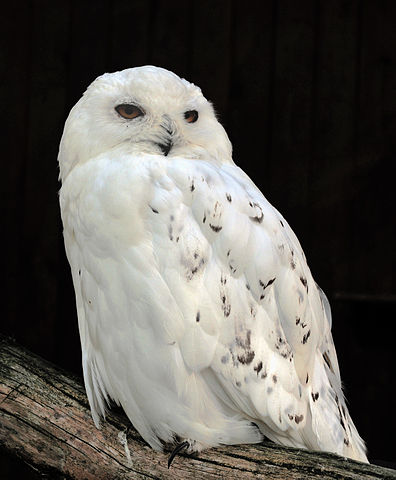
\includegraphics[width=0.3\textwidth]{images/396px-Bubo_scandiacus_(Linnaeus,_1758)_Male.jpg}
\caption{Eine Schneeeule \cite{ref3}}
\end{wrapfigure}{} 
Lamports Entwicklung von LaTeX endete gegen 1990 mit der Version 2.09.[2] Die aktuelle Version LaTeX wurde ab 1989 von einer größeren Zahl von Autoren um Frank Mittelbach, Chris Rowley und Rainer Schöpf entwickelt. Wesentliche Erweiterungen von Lamports Versionen bestanden in einem „vierdimensionalen“ Mechanismus für das Umschalten zwischen Zeichensätzen („New Font Selection Scheme“, „NFSS“), in einem komplexeren Mechanismus für das Einlesen von Zusatzpaketen und in einer entsprechenden „Paketschreiberschnittstelle“ für die Erstellung und Dokumentation auf LaTeX aufbauender Makropakete. Die beiden Entwicklungsstufen von LaTeX sind nicht kompatibel.
LaTeX 2 ist seit Mitte der 1990er Jahre die am weitesten verbreitete Methode, TeX zu verwenden.\\
Im Gegensatz zu anderen Textverarbeitungsprogrammen, die nach dem What-you-see-is-what-you-get-Prinzip funktionieren, arbeitet der Autor mit Textdateien, in denen er innerhalb eines Textes anders zu formatierende Passagen oder Überschriften mit Befehlen textuell auszeichnet. Das Beispiel unten zeigt den Quellcode eines einfachen LaTeX-Dokuments. Bevor das LaTeX-System den Text entsprechend setzen kann, muss es den Quellcode verarbeiten. Das dabei von LaTeX generierte Layout gilt als sehr sauber, sein Formelsatz als sehr ausgereift. Außerdem ist die Ausgabe u. a. nach PDF, HTML und PostScript möglich. LaTeX eignet sich insbesondere für umfangreiche Arbeiten wie Diplomarbeiten und Dissertationen, die oftmals strengen typographischen Ansprüchen genügen müssen. Insbesondere in der Mathematik und den Naturwissenschaften erleichtert LaTeX das Anfertigen von Schriftstücken durch seine komfortablen Möglichkeiten der Formelsetzung gegenüber üblichen Textverarbeitungssystemen. Das Verfahren von LaTeX wird auch mit WYSIWYAF (What you see is what you asked for.) umschrieben. 

\newpage

\section{Zwei Bilder \cite{ref4}}

Es folgen nun zwei Bilder die nebeneinander positioniert sind. Die Bilder befinden sich dabei
%in einer \textit{figure} Umgebung und selbst jeweils in einer \textit{subfigure} Umgebung. Die Anmerkungen wurden mithilfe des Paketes \textit{caption} und \textit{subcaption} ermöglicht. Los geht es!
\vspace{10pt}
\begin{figure}[h!]
	\centering
	\begin{subfigure}{.5\textwidth}
		\centering
		
\includegraphics[width=.9\linewidth]{images/Nederlands_verkeersbord_C4_(links).png}
		\caption{Bild A}
		
	\end{subfigure}%
	\begin{subfigure}{.5\textwidth}
		\centering
		
\includegraphics[width=.9\linewidth]{images/Nederlands_verkeersbord_C4_(rechts).png}
		\caption{Bild B}
		
	\end{subfigure}
	\caption{Gesamtbildunterschrift}

\end{figure}


\newpage

\begin{thebibliography}{mmmmmmm}
	\bibitem{ref1} Theater Freiburg (2008, Feb. 08) \textit{Beispieltext mit 1000 Wörtern} [Online].\newline \url{https://theaterfreiburg.wordpress.com/2008/02/28/beispieltext-mit-1000-worten/} 
	
	\bibitem{ref2} Wikipedia (2016, Jun. 21) \textit{LaTeX} [Online].\newline \url{https://de.wikipedia.org/wiki/LaTeX} 
	
	\bibitem{ref3} Wikipedia (2016, Oct. 01) \textit{Schnee-Eule, Männchen} [Online]. \newline
	\url{https://de.wikipedia.org/wiki/Schnee-Eule#/media/File:Bubo_scandiacus_(Linnaeus,_1758)_Male.jpg}
	
	\bibitem{ref4} Wikipedia (2007, Aug. 07) \textit{Nederlands verkeersbord C4} [Online]. \newline
	\url{https://de.wikipedia.org/wiki/Datei:Nederlands_verkeersbord_C4_(rechts).svg}
	
	
	
\end{thebibliography}



\end{document}